\newpage
\chapter{Configuración del clúster}
\label{ch:capitulo3.tex}

\begin{FraseCelebre}
	\begin{Frase}
		Tenemos que fabricar máquinas que nos permitan seguir fabricando máquinas, porque lo que no va a hacer nunca la máquina es fabricar máquinas
	\end{Frase}
	\begin{Fuente}
	M.Rajoy
	\end{Fuente}
\end{FraseCelebre}

Al lo largo de este capítulo se detallan los pasos necesarios para la correcta configuración del sistema. En cada apartado se especifican los pasos a seguir para la configuración e instalación de los distintos servidores y software necesarios. 

\section{Virtualización del sistema}
\label{makereference3.1}
\paragraph{}

Debido a la gran cantidad de componentes necesarios para el desarrollo del proyecto, la necesidad de realizar el montaje y desmontaje de forma manual de estos y la dificultad en el acceso y configuración de cada uno de los nodos que lo componen decidimos realizar una virtualización del sistema para minimizar los problemas antes descritos. Así, al disponer de un entorno virtual, el cual, replica el clúster real, se minimiza el tiempo necesario para la configuración de los distintos servicios y servidores del sistema operativo y sirve, a su vez, como banco de pruebas para el desarrollo de software.

Para ello, hemos utilizamos \textit{VMware workstation 12} como plataforma de software de virtualización y una \textbf{imagen} de Raspbian basada en \textit{Debian Stretch} , la cual se encuentra disponible en la página oficial de Raspberry Pi\footnote{\url{http://downloads.raspberrypi.org/raspbian/images/}}. Aunque el sistema del clúster parte de una versión diferente de Debian, el sistema de carpetas y, sobre todo, la instalación de \textbf{SIMCAN}, es similar al del entorno real.

En el repositorio en \textit{Github} existe una réplica del sistema de carpetas tanto para el servidor como para los nodos esclavo. Cada una de las carpetas y ficheros modificados en el sistema durante la configuración del sistema quedan reflejados en el repositorio, disponiendo así de un listado en forma de árbol de todas las configuraciones necesarias para el correcto funcionamiento de este.

\begin{figure}[H]
	\centering
  	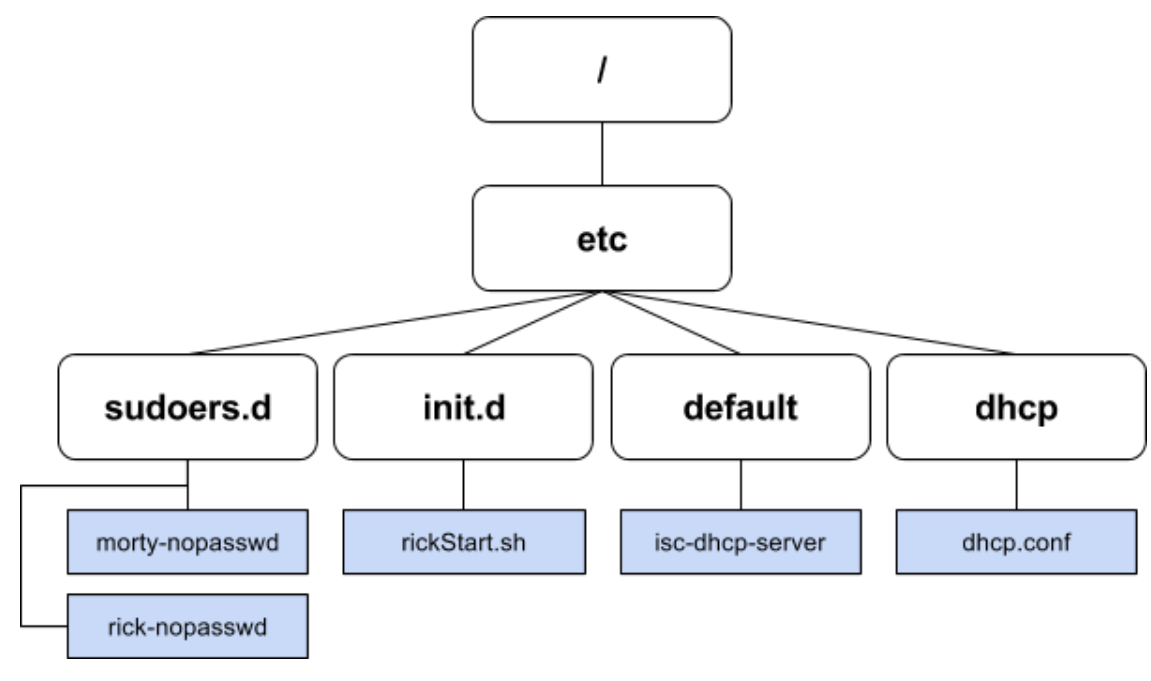
\includegraphics[width=110mm]{pics/sistemadearchivos.PNG}
   	\caption[Sistema de archivos]{Sistema de archivos del repositorio}
   \label{figure3.1}
\end{figure}

\section{Sistema centralizado}
\label{makereference2.6}

Hemos decidido realizar nuestro sistema con una arquitectura de cluster computing centralizado para obtener más rendimiento y paralelizar aplicaciones, de este modo aprovechamos todos los recursos del cluster en su ejecución.

Disponemos de un nodo maestro que contiene el front-end y el back-end y realiza el envío de las peticiones a los esclavos, es escalable pudiendo incorporar nuevos nodos a la red, además ofrece una mayor seguridad sobre los sistemas descentralizados ya que todo el procesamiento es controlado a través de una localización central.

\begin{figure}[H]
	\centering
  	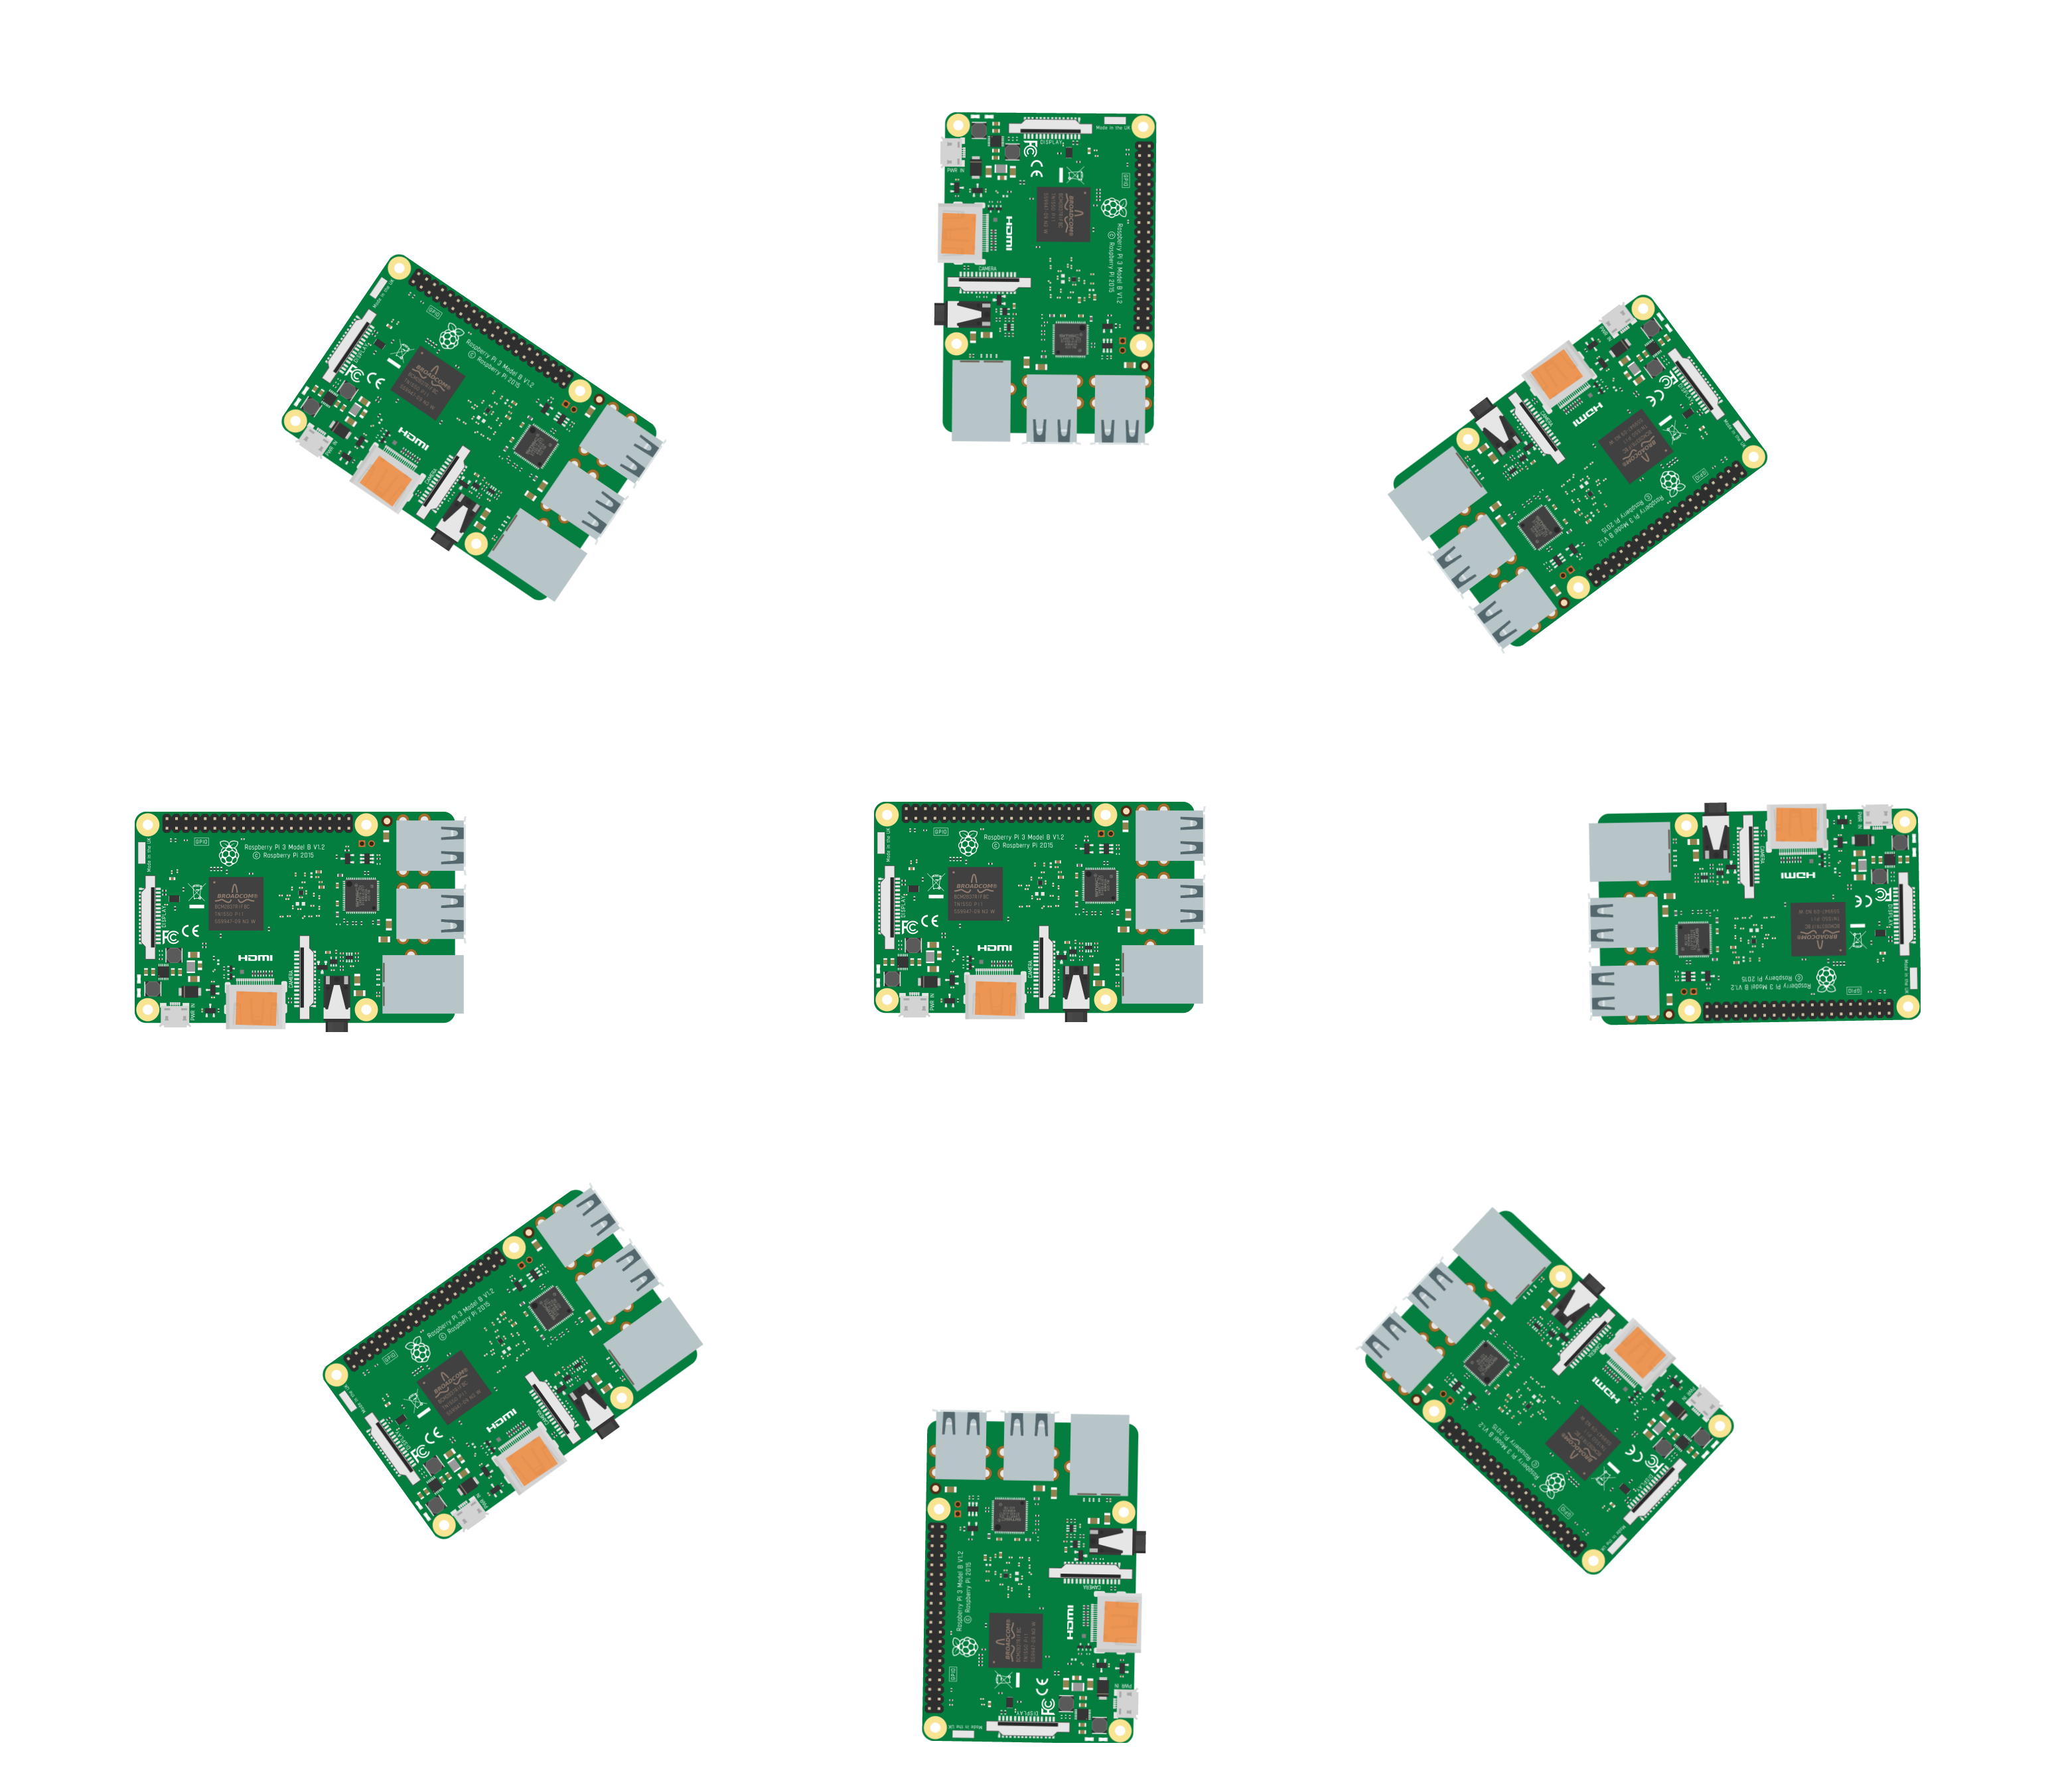
\includegraphics[width=100mm]{pics/centralizado.png}
   	\caption[Sistema centralizado]{Sistema centralizado}
   \label{figure2.6}
\end{figure}

\section{Arquitectura del Clúster}
\label{makereference3.3}
\paragraph{}

El clúster está dividido en dos partes diferenciadas. Por un lado, el \textit{front-end}, servidor, nodo del clúster que tiene instalado el software de \textbf{SIMCAN}, además de ofrecer los servicios de \textbf{NFS}, \textbf{DHCP} y \textbf{SSH} entre otros nodos como muestra la figura \ref{figure3.2}. Además, el punto de comunicación con el exterior, por ello dispone de una tarjeta de red adicional.

\begin{figure}[H]
	\centering
  	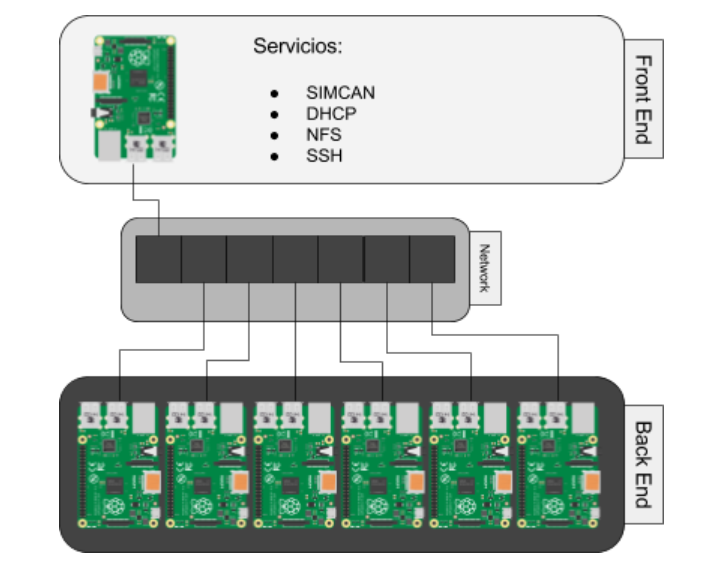
\includegraphics[width=90mm]{pics/servidores.PNG}
   	\caption[Esquema]{Esquema del sistema}
   \label{figure3.2}
\end{figure}

Por otro lado, en el \textit{back-end}, disponemos de varios nodos esclavo que disponen únicamente del sistema Debian Jessie, así como de bibliotecas necesarias para realizar las operaciones de cómputo.

\section{Configuración de la red}
\label{makereference3.4}
\paragraph{}

La configuración de la red se realiza mendiante DHCP, en este caso utilizaremos......

La red en la que trabajamos es la \textit{172.16.111.0/24}. El front end tiene asignada la dirección \textit{172.16.111.1/24}, y ejerce de servidor sobre el resto de nodos, encargándose del reparto de direcciones, como se muestra en la figura \ref{figure3.3}.

\begin{figure}[H]
	\centering
  	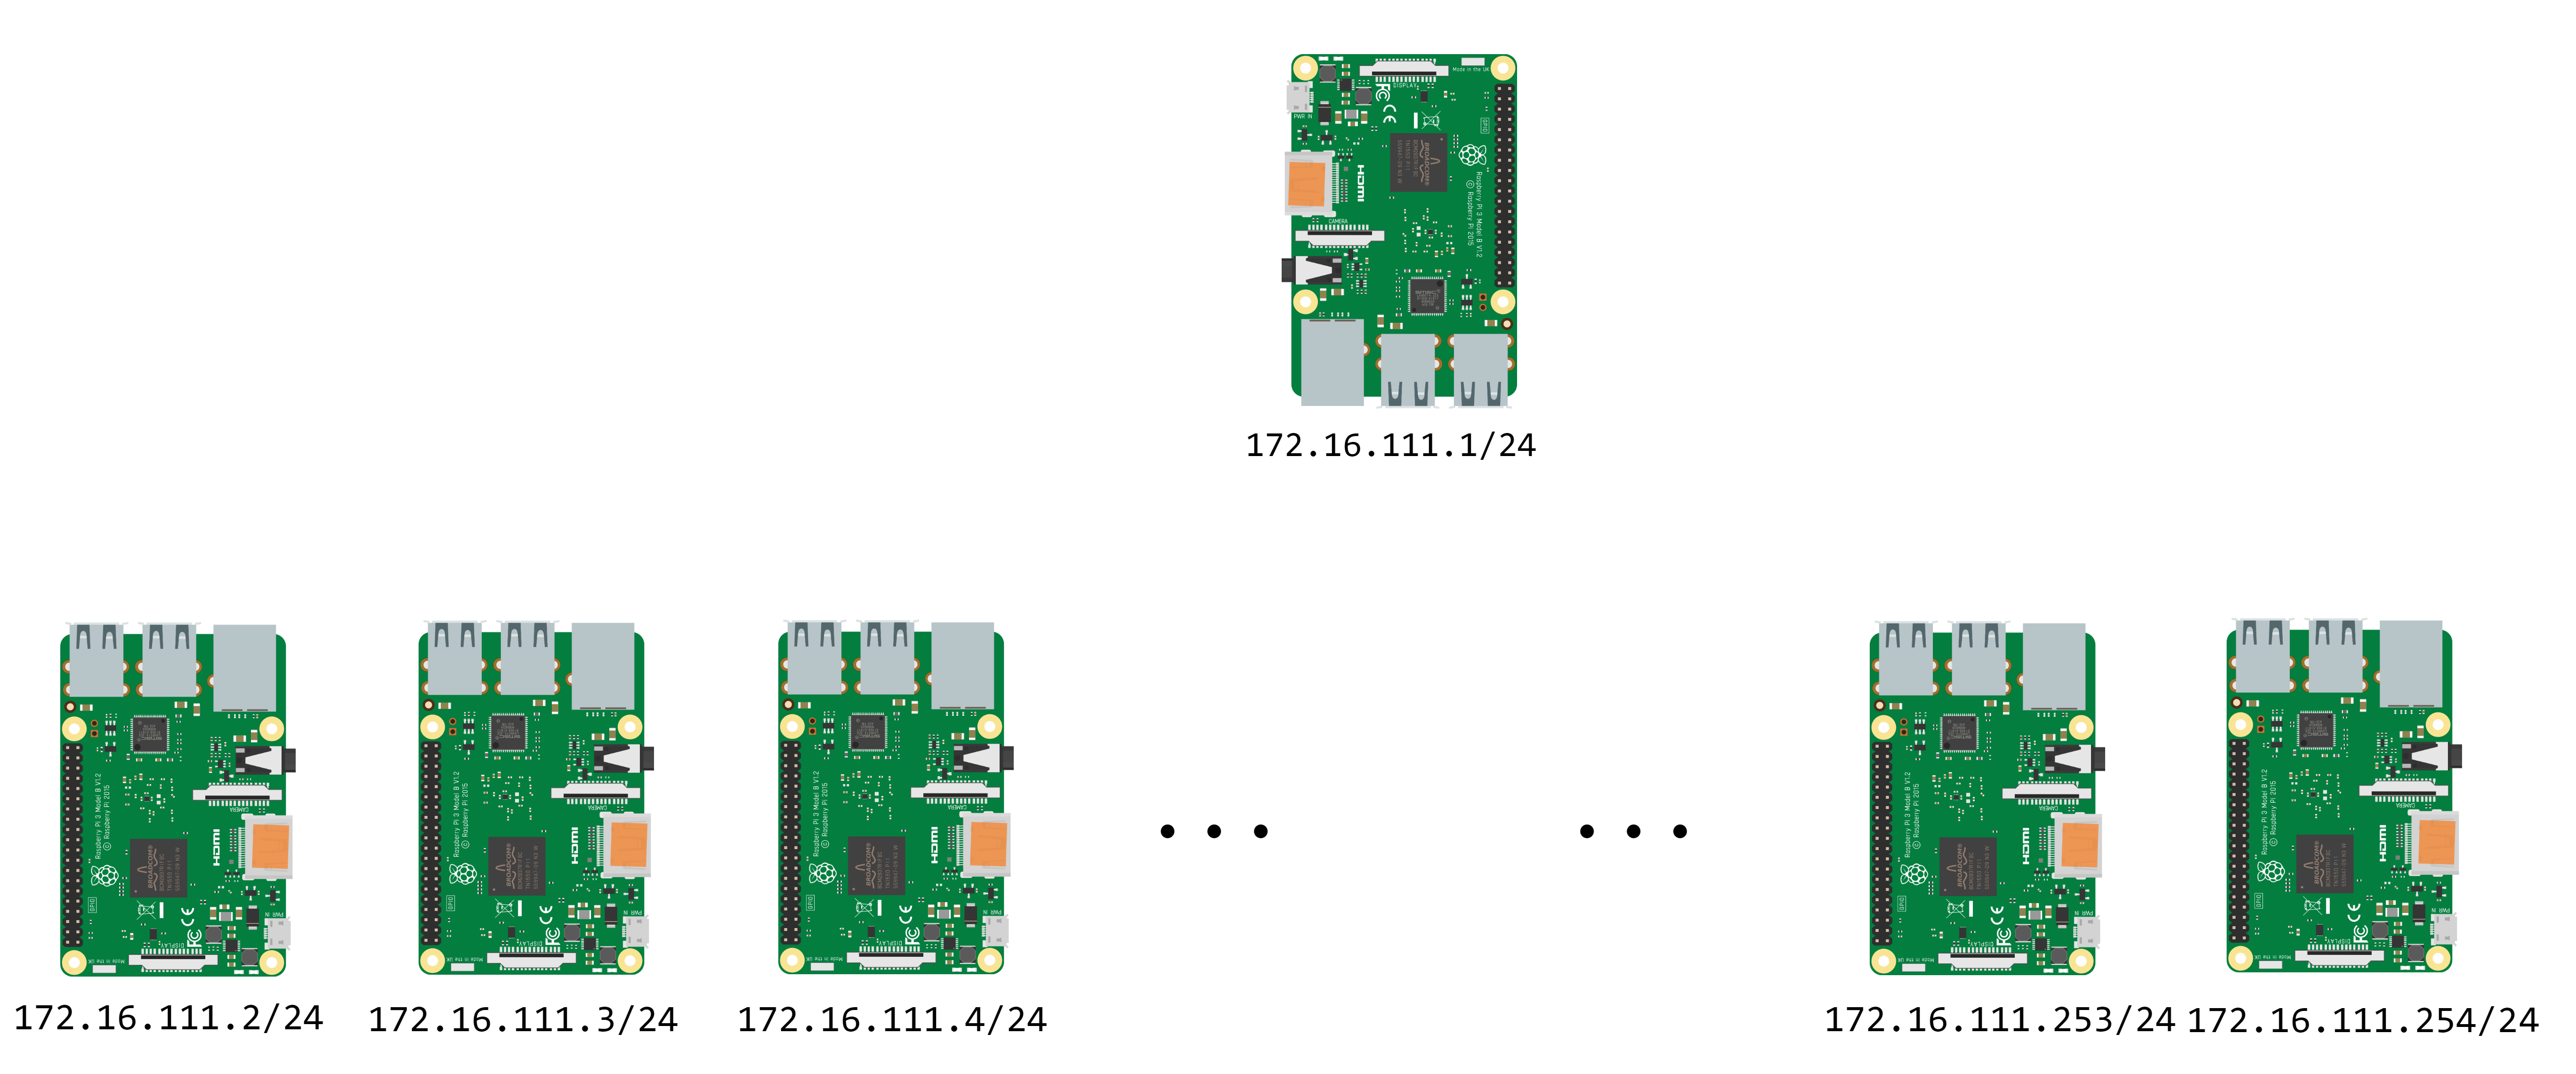
\includegraphics[width=120mm]{pics/dhcpdos.png}
   	\caption[Servidor DHCP]{Servidor DHCP}
   \label{figure3.3}
\end{figure}

Gracias al uso del protocolo \textbf{DHCP} evitamos tener que asignar manualmente direcciones a todos los nodos, sin embargo, es más útil en la práctica que cada uno de los nodos disponga de la misma dirección el máximo tiempo posible.

¿¿Por qué??

Para ello, en el fichero \textbf{/etc/dhcp/dhcpd.conf}, hemos establecido el parámetro \textbf{default-lease-time} que determina el tiempo de concesión de que el servidor asigna a cada nodo en su máximo valor. El tiempo por defecto (7776000 expresado en segundos) será de noventa días.

\begin{lstlisting}[language=c,frame=single,numbers=none]
      ...
      default-lease-time	7776000;
      ...
\end{lstlisting}

Los servicios ofrecidos por el nodo maestro de cara al \textit{front-end} están disponibles a través de su segunda tarjeta de red, configurada para obtener una dirección IP desde un \textbf{ISP}.

\subsection{Configuración de DHCP}
\paragraph{}

Instalación de paquetes en el servidor

\begin{lstlisting}[language=c,frame=single,numbers=none]
  1	sudo apt-get update
  2	sudo apt-get install isc-dhcp-server
\end{lstlisting}

Editar fichero \textbf{/etc/default/isc-dchp-server}

\begin{lstlisting}[language=c,frame=single,numbers=none]
  3	sudo nano /etc/default/isc-dchp-server
  4	INTERFACES = eth0
\end{lstlisting}

Editar fichero \textbf{/etc/network/interfaces}

\begin{lstlisting}[language=c,frame=single,numbers=none]
  5	nano /etc/network/interfaces
  6	source-directory /etc/network/interfaces.d

  auto eth0	
  iface eth0 inet static
  address 172.16.111.106
  netmask 255.255.255.0
  network 192.168.100.0
  gateway 172.16.111.105

  allow-hotplug wlan0
  iface wlan0 inet manual
      wpa-conf /etc/wpa_supplicant/wpa_supplicant.conf

  allow-hotplug wlan1
  iface wlan1 inet manual
      wpa-conf /etc/wpa_supplicant/wpa_supplicant.conf
\end{lstlisting}

Editar fichero de configuración \textbf{/etc/dhcp/dhcpd.conf}

Incluir la siguiente configuración al final del fichero:
\begin{lstlisting}[language=c,frame=single,numbers=none]
  subnet 172.16.111.0 netmask 255.255.255.0{
      range 172.16.111.106	172.16.111.255;
      option domain-name-servers 8.8.8.8, 4.4.4.4;
      option routers		172.16.111.105;
  }
  host Rick{
      hardware ethernet <dir MAC del servidor>
      fixed-address 172.16.111.110;
  }
\end{lstlisting}

Activación de la red eth0 y reinicio

\begin{lstlisting}[language=c,frame=single,numbers=none]
  7	sudo ifconfig eth0 up
  8	sudo reboot now 
\end{lstlisting}

Arranque del servicio DHCP

\begin{lstlisting}[language=c,frame=single,numbers=none]
  9	sudo /usr/sbin/dhcpd
\end{lstlisting}

Comprobación del correcto funcionamiento del sistema

\begin{lstlisting}[language=c,frame=single,numbers=none]
  10	ps -ef | grep dhcpd
\end{lstlisting}

Opcionalmente se pueden mostrar las máquinas conectadas al servicio mediante la orden

\begin{lstlisting}[language=c,frame=single,numbers=none]
  11	cat /var/lib/dhcp/dhcp.leases 
\end{lstlisting}

\subsection{Network File System (NFS)}
\label{makereference3.5}
\paragraph{}

Como se destacaba anteriormente, el front-end es el único que dispone de una versión de \textbf{SIMCAN} instalada, con esto se evitan problemas de versiones y es mas sencillo realizar actualizaciones, esta configuración ofrece la posibilidad de que la labor del los nodos esclavo sea únicamente la de realizar el procesamiento de datos. Mediante \textbf{NFS}, el nodo servidor comparte su carpeta /home/ durante el arranque del sistema. De esta forma, el resto de nodos esclavo realizan el montaje de este directorio compartido en red en su propio directorio /home/, creando así un único punto de acceso compartido en red del que se pueden extraer los ejecutables sin la necesidad de disponer de \textbf{SIMCAN} instalado. El front-end se encarga de realizar la compilación los ficheros \textit{.ned} y pone a disposición del resto de nodos los ejecutables.

Es necesario que todos los nodos de la red tengan un mismo usuario común para conseguir una correcta sincronización, de igual manera hay que mantener un estricto control de los permisos de cada uno de los nodos esclavo tanto a nivel interno como de cara al servidor.

\subsection{Instalación de NFS}
\paragraph{}

PARRAFO DE INTRODUCCION.....

Instalar paquetes en el servidor

\begin{lstlisting}[language=c,frame=single,numbers=none]
  1	sudo apt-get update
  2	sudo apt-get install nfs-kernel-server
\end{lstlisting}

Editar fichero de configuración \textbf{/etc/exports} en servidor
\begin{lstlisting}[language=c,frame=single,numbers=none]
	Incluir al final del fichero el directorio a compartir:
	Ruta de carpeta
	Dirección IP de máquina destino / permisos

	Ejemplo: /home/morty 172.16.111.0/24(rw,no_subtree_check)
\end{lstlisting}

Instalación de paquetes en el cliente
\begin{lstlisting}[language=c,frame=single,numbers=none]
  Instalados por defecto en raspBian
  3	sudo apt-get update
  4	sudo apt-get install build-essential gcc g++ bison flex perl  tcl-dev tk-dev libxml2-dev zlib1g-dev default-jre doxygen graphviz libwebkitgtk-1.0-0 openmpi-bin libopenmpi-dev libpcap-dev
\end{lstlisting}

Ejecutar cambios realizados en el servidor

\begin{lstlisting}[language=c,frame=single,numbers=none]
  5	sudo exportfs -a
  6	sudo mount 172.16.111.x:/home/morty /home/morty
      172.16.111.x es la dirección ip de servidor
\end{lstlisting}

Reiniciar servicios 
\begin{lstlisting}[language=c,frame=single,numbers=none]
  7	sudo /etc/init.d/rpcbind restart
  8	sudo /etc/init.d/nfs-kernel-server restart
\end{lstlisting}

Es necesaria una configuración extra para el funcionamiento de NFS, pare ello modificamos permisos de la maquina cliente:
\begin{enumerate}

\item El usuario de la máquina ha de ser sudoer. La carpeta compartida debe tener permisos de lectura, escritura y ejecución \textbf{(LWX)}:

\begin{lstlisting}[language=c,frame=single,numbers=none]
    chmod -R 0777 scenario
\end{lstlisting}

\end{enumerate}
\subsection{Creación y ejecución del servidor NFS como un  \textit{daemon} del sistema}
\paragraph{}

Para evitar tener que realizar el arranque del servidor de forma manual es recomendable crear un \textit{daemon} e incluirlo en el directorio \textbf{/etc/init.d} para que se ejecute con el arranque del sistema de forma automática.

Contenido del script:

\begin{lstlisting}[language=c,frame=single,numbers=none]
	#!/bin/bash
	### BEGIN INIT INFO
	# Provides:		M.Romero && D.Quinones
	# Required-start:	$syslog
	# Required-stop:	$syslog
	# Default-Start:	2 3 4 5
	# Default-Stop:		0 1 6
	# Short-Description:	Inicialización de servicios nfs
	# Description:	
	### END INIT INFO

	sudo exportfs -a
	sudo /etc/init.d/rpcbind restart
	sudo /etc/init.d/nfs-kernel-server restart

  # El orden de estos últimos comandos es esencial
\end{lstlisting}

El siguiente cuadro muestra los pasos a seguir para lanzar el script como un \textit{daemon} del sistema:

\begin{lstlisting}[language=c,frame=single,numbers=none]
  10	chmod +x nombre_del_script.sh
  11	cp nombre_del_script.sh /etc/init.d/
  12	cd /etc/init.d
  13	update-rc.d nombre_del_script.sh defaults
\end{lstlisting}

\section{Instalación de Omnet, Inet y SIMCAN}
\label{makereference3.6}
\paragraph{}
Antes de poder instalar el software \textbf{SIMCAN} es necesario realizar la instalación previa framework \textbf{Omnet++} en su versión 4.6. Además de la suite \textbf{Inet}, que implementa modelos de código abierto \textbf{Omnet++} para redes cableadas, inalámbricas y móviles.

Debido a la baja potencia de la Raspberry, ésta no es capaz de lanzar la aplicación de forma gráfica. Esto supone un problema a la hora de realizar la instalación del software. Es por esto que todas las instalaciones han de realizarse a través del terminal. Esto afecta principalmente a la instalación de \textbf{Inet}, ya que las principales guías de instalación disponibles en las webs oficiales parten siempre del entorno gráfico de \textbf{Omnet++}.

Durante el desarrollo del proyecto se han desarrollado una serie de guías para la instalación y configuración que se desglosarán el el siguiente apartado.

\subsection{Instalación de Omnet}
\paragraph{}

Descargar los \textit{tar.gz}  de Omnet 4.6, Inet, simcan.tar.
Esta última (simcan) incluye las bibliotecas que se necesitan para la compilación.
Copiar los archivos \textit{.tar} de Omnet e Inet en \textbf{/pi} y descomprimir. Desde el directorio \textbf{/pi} ejecuta los siguientes comandos:

\begin{lstlisting}[language=c,frame=single,numbers=none]
  1	sudo apt-get update
  2	sudo apt-get install build-essential gcc g++ bison flex perl  tcl-dev tk-dev libxml2-dev zlib1g-dev default-jre doxygen graphviz libwebkitgtk-1.0-0 openmpi-bin libopenmpi-dev libpcap-dev
  3	sudo apt-get install gnome-color-chooser
  4	cd omnetpp-4.6
  5	. setenv
  6	./configure
  7	make
  * Opcionalmente podemos utilizar el comando make -j 'numero de cores'
  para paralelizar el compilado del proyecto
\end{lstlisting}

\subsection{Instalación de Inet}
\paragraph{}

INCLUIR FRASE DE INTRODUCCIÓN

Crear un directorio nuevo en \textbf{/omnet-4.6} llamado \textit{proyect}, copiar en el directorio \textbf{Inet} descomprimido y ejecutar:

\begin{lstlisting}[language=c,frame=single,numbers=none]
  8	sudo apt-get install libavcodec-dev libavformat-dev
  9	make makefiles
  10	make
  * Opcionalmente podemos utilizar el comando make -j 'numero de cores'
  para paralelizar el compilado del proyecto
\end{lstlisting}

\subsection{Instalación de SIMCAN}
\paragraph{}

Copia el directorio de \textbf{simcan} a \textbf{/projects} y ejecuta los siguientes comandos:

\begin{lstlisting}[language=c,frame=single,numbers=none]
  11	export omnetpp_root=$HOME/morty/omnnetpp-4.6
  12	export INET_HOME=$omnetpp_root/projects/inet
  13	export SIMCAN_HOME=$omnetpp_root/projects/simcan
  14	export LD_LIBRARY_PATH=$omnetpp_root/lib:$LD_LIBRARY_PATH 
  15	export PATH=omnetpp_root/bin:$PATH
  16	make makefiles
  17	make
  * Opcionalmente podemos utilizar el comando make -j 'numero de cores'
  para paralelizar el compilado del proyecto
  Enjoy!
\end{lstlisting}

\subsection{Problemas}
\paragraph{}

\begin{enumerate}

\item No se encuentra el fichero \textbf{TCPCommand\_m.h}
\begin{lstlisting}[language=c,frame=single,numbers=none]
	cp /home/pi/omnetpp-4.6/proyects/inet/src/transport/contract/TCPCommand_m.h /home/pi/omnetpp-4.6/proyects/simcan/src/Messages/TCPCommand_m.h
\end{lstlisting}

\item Error al ejecutar \textbf{run\_simcan}

\begin{lstlisting}[language=c,frame=single,numbers=none]
	chmod +x /simcan/src/run_sincam
\end{lstlisting}

\end{enumerate}


\section{Configuraciones derivadas de la arquitectura}
\label{makereference3.7}
\paragraph{}

Como se ha explicado anteriormente, la arquitectura elegida distribuye la potencia a todos los nodos del clúster desde una misma fuente de alimentación. Debido a la menor cantidad de recursos y servicios que han de ofrecer los nodos esclavo, éstos tienen una carga del sistema ligeramente más rápida que la del nodo maestro. Por ello, se pueden producir problemas de sincronización de servicios, más concretamente, en el montaje de sistemas de ficheros compartidos en red por \textbf{NFS}, el cual es crítico para el funcionamiento general del sistema. Para solucionar este problema se han realizado modificaciones a fin de conseguir acelerar la carga del nodo maestro y ralentizar la del resto.

\subsection{Modificación del GRUB}
\paragraph{}

Una de las soluciones más sencillas para resolver el problema de sincronización consiste en aumentar el tiempo por defecto del \textit{grub} de los nodos esclavo ya que la carga del sistema se produce cuando éste termina. Para ello únicamente hay que modificar la opción \textbf{GRUBTIMEOUT} en el fichero \textbf{/etc/default/grub}. 
En las pruebas realizadas durante la virtualización del sistema se comprobó que estableciendo un retardo de veinticinco segundos era suficiente para que el nodo maestro realizase la carga completa del sistema. Sin embargo, queda por comprobar que en el entorno real esto se sigue produciendo.

Contenido del fichero \textbf{/etc/default/grub} de un nodo esclavo:

\begin{lstlisting}[language=c,frame=single,numbers=none]
  GRUB_DEFAULT=0
  GRUB_TIMEOUT=25
  GRUB_DISTRIBUTOR=`lsb_release -i -s 2> /dev/null || echo Debian`
  GRUB_CMDLINE_LINUX_DEFAULT="quiet splash plymouth.ignore-serial-consoles"
  GRUB_CMDLINE_LINUX=""
\end{lstlisting}

\subsection{Habilitar arranque automático de un usuario}
\paragraph{}

Para modificar el usuario de arranque por defecto es necesario realizar los siguientes cambios en el fichero \textbf{/etc/lightdm/lightdm.conf}
\begin{lstlisting}[language=c,frame=single,numbers=none]
  autologin-user = nombre_de_usuario
\end{lstlisting}

\subsection{Forzar el arranque sin HDMI}
\paragraph{}

En ocasiones \textit{Raspbian Jessie} no realiza la carga del sistema operativo si el conector \textbf{HDMI} no está acoplado en la Raspberry, para forzar el arranque del sistema es necesario modificar el archivo \textbf{/boot/config.txt}

\begin{lstlisting}[language=c,frame=single,numbers=none]
	#Arranque sin HDMI
    hdi_force_hotplug = 1
\end{lstlisting}

\section{Seguridad}
\label{makereference3.8}
\paragraph{}
Por defecto, en las distribuciones de \textit{Debian Jessie} existentes en los repositorios oficiales de raspberry.org existe...
Vienen configurados usuarios por defecto
Root no tiene contraseña
Hay que eliminar a pi como superuser
Sólo dejar morty como superuser en maestro pero no en esclavos

\section{Eliminar usuarios y permisos}
\label{makereference3.9}
\paragraph{}
UID, todos han de tener el mismo, permisos en maestro, esclavo
Inicialización del sistema mediante scripts


